\documentclass[12pt]{article}
\usepackage[utf8]{inputenc}
\usepackage[margin=1in]{geometry}
\usepackage{amsmath}\usepackage{amssymb}\usepackage{multicol}\usepackage{enumitem}
\usepackage{pgfplots}\pgfplotsset{compat=1.17}
\setlength{\parindent}{0pt}
\begin{document}

\fbox{\parbox{0.97\linewidth}{\small\textbf{Final answers} (record here --- graded on the answer; show your work):\\[6pt]1.~\underline{\hspace{1.5cm}}\quad 2.~\underline{\hspace{1.5cm}}\quad 3.~\underline{\hspace{1.5cm}}\quad 4.~\underline{\hspace{1.5cm}}\quad 5.~\underline{\hspace{1.5cm}}\quad 6.~\underline{\hspace{1.5cm}}\quad 7.~\underline{\hspace{1.5cm}}\quad 8.~\underline{\hspace{1.5cm}}\quad 9.~\underline{\hspace{1.5cm}}\quad 10.~\underline{\hspace{1.5cm}}\quad 11.~\underline{\hspace{1.5cm}}}}
\vspace{0.35cm}

\begin{center}{\Large \textbf{Identify the family, domain, and range}}\end{center}\vspace{0.2cm}
% Identify the family, domain, and range
\textbf{Example (Identify the family, domain, and range):}

$f(x)=\dfrac{1}{x}$ is the \textbf{reciprocal} parent. A denominator can't be $0$, so the domain is $x\ne 0$; the graph never touches $y=0$ either, so the range is $y\ne 0$.

\begin{center}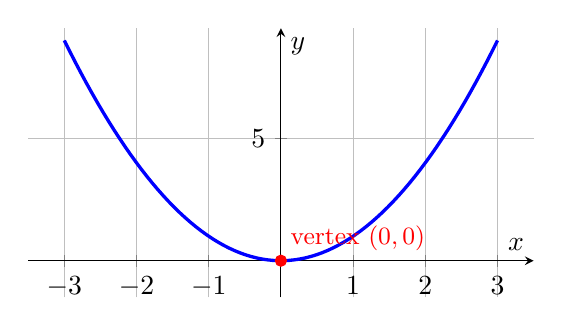
\begin{tikzpicture}
\begin{axis}[axis lines=middle,xlabel=$x$,ylabel=$y$,xmin=-3.5,xmax=3.5,ymin=-1.5,ymax=9.5,width=8cm,height=5cm,grid=both,samples=80]
\addplot[very thick,blue,domain=-3:3]{x^2};
\addplot[only marks,mark=*,red] coordinates {(0,0)};
\node[above right,red,font=\small] at (axis cs:0,0) {vertex $(0,0)$};
\end{axis}\end{tikzpicture}\end{center}
{\small\centering $y=x^{2}$ --- the quadratic parent function.\par}
\vspace{0.2cm}\hrule\vspace{0.35cm}
\textbf{Directions: Name the parent family, then give the domain and range.}

\begin{multicols}{2}
\begin{enumerate}[label=\textbf{\arabic*.}, start=1, itemsep=2cm]
  \item $\displaystyle f(x)=x$
  \item $\displaystyle f(x)=x^{2}$
  \item $\displaystyle f(x)=x^{3}$
  \item $\displaystyle f(x)=|x|$
  \item $\displaystyle f(x)=\sqrt{x}$
  \item $\displaystyle f(x)=\dfrac{1}{x}$
\end{enumerate}
\end{multicols}
\vspace{0.25cm}\hrule\vspace{0.35cm}

\begin{center}{\Large \textbf{Match a shifted equation back to its parent family}}\end{center}\vspace{0.2cm}
% Match a shifted equation back to its parent family
\textbf{Example (Match a shifted equation back to its parent family):}

$g(x)=\sqrt{x}+4$ still has a radical, so its parent family is \textbf{square root} (the $+4$ just shifts it later).

\vspace{0.2cm}\hrule\vspace{0.35cm}
\textbf{Directions: Even though these are shifted, name the ORIGINAL parent family only.}

\begin{multicols}{2}
\begin{enumerate}[label=\textbf{\arabic*.}, start=7, itemsep=1.3cm]
  \item $\displaystyle g(x)=(x-2)^{2}$
  \item $\displaystyle g(x)=|x+1|-3$
  \item $\displaystyle g(x)=\dfrac{1}{x-5}$
  \item \textbf{(challenge)}\ $\displaystyle g(x)=(x+3)^{3}+1$
\end{enumerate}
\end{multicols}

\vspace{0.2cm}\hrule\vspace{0.3cm}
\textbf{Challenge} (same sheet):\\[4pt]
\begin{enumerate}[label=\textbf{\arabic*.}, start=11, itemsep=2.2cm]
  \item Sketch all 6 parent functions from memory on one set of axes, labeling each with its equation.
\end{enumerate}

\newpage

\begin{center}{\Large \textbf{Answer Key --- fully worked}}\end{center}
\vspace{0.25cm}
\textbf{Procedure:} Look for a root symbol, absolute value bars, or an exponent to identify the family.; Ignore any added/subtracted numbers outside --- they only shift the graph, not the family.; Check for a denominator or a radical: these create domain restrictions.; State domain first, then determine range from the graph's lowest or highest point..\\[8pt]
\begin{enumerate}[label=\textbf{\arabic*.},itemsep=7pt]
  \item Linear; domain: all real numbers; range: all real numbers
  \item Quadratic; domain: all real numbers; range: $y\ge 0$
  \item Cubic; domain: all real numbers; range: all real numbers
  \item Absolute value; domain: all real numbers; range: $y\ge 0$
  \item Square root; domain: $x\ge 0$; range: $y\ge 0$
  \item Reciprocal; domain: $x\ne 0$; range: $y\ne 0$
  \item Quadratic (the $(x-2)^2$ is still squared, just shifted right)
  \item Absolute value (the bars are still there, just shifted)
  \item Reciprocal (still a fraction with $x$ in the denominator)
  \item Cubic --- the exponent of 3 on $(x+3)$ shows this came from the cubic parent, just shifted left 3 and up 1
  \item Six correct sketches on one grid: $y=x$ (straight line through origin, slope 1); $y=x^{2}$ (U-shaped parabola, vertex $(0,0)$); $y=x^{3}$ (S-shaped curve through origin, rising left to right); $y=|x|$ (V-shape, vertex $(0,0)$, opening up); $y=\sqrt{x}$ (half-parabola starting at $(0,0)$, in the first quadrant only); $y=\dfrac{1}{x}$ (two hyperbola branches in quadrants I and III, never touching either axis). Each curve labeled with its equation; $\sqrt{x}$ and $1/x$ should visibly show their restricted domains.
\end{enumerate}

\end{document}